%----------------------------------------------------
%
% Title:  Traverso 0.40.0
% Author: Remon Sijrier, Nicola Doebelin
% Date:   Januar 13, 2007
%
%----------------------------------------------------
% Created with TeXwiz 2.0.0
%----------------------------------------------------

\documentclass[a4paper,
               12pt,
               pdftex,
               twoside,
               smallheadings,
               headinclude,
               headsepline,
               DIV16,
               BCOR10mm
               ]{scrreprt}

\usepackage{mathpazo}
\usepackage[scaled=.95]{helvet}
\usepackage{courier}
\linespread{1.05}
\usepackage[latin1]{inputenc}
\usepackage{calc}
\usepackage{graphicx}
\usepackage{subfigure}
\usepackage{amssymb}
\usepackage{booktabs}
\usepackage{pdfpages}

%---------------- Page style options ----------------

\usepackage[automark]{scrpage2}
\pagestyle{scrheadings}

\setcapindent{1em}

%-------------- Custom Markup Commands --------------

\newcommand*{\FigB}{fig.}      % "fig." as used in brackets
\newcommand*{\FigT}{figure}    % "figure" as used in running text
\newcommand*{\FigsT}{figures}  % "figures" (plural) in running text
\newcommand*{\TabB}{tab.}      % "tab." as used in brackets
\newcommand*{\TabT}{table}     % "table" as used in running text
\newcommand*{\TabsT}{tables}   % "tables" (plural) used in running text

\newcommand*{\sact}[1]{$<$#1$>$} % single click action
\newcommand*{\dact}[1]{$\ll$#1$\gg$} % double click action
\newcommand*{\hact}[1]{{[#1]}} % single hold action

\newcommand*{\Version}{0.5.0} % The current version of traverso
\newcommand*{\Ubuntu}{8.10} % The current Ubuntu version

%---------------- PDF output options ----------------

\pdfoutput=1
\usepackage{thumbpdf}
\usepackage{pdflscape}
\usepackage[bookmarks]{hyperref}
\pdfimageresolution=300
\pdfcompresslevel=9

\pdfinfo{
/Title(Traverso 0.5.0)
/Creator(TeX)
/Producer(PdfTeX)
/Author(Nicola Doebelin)
/CreationDate(D:20070113145749)
/Subject(Traverso 0.5.0)}

%----------------------------------------------------

\renewcommand{\floatpagefraction}{0.6}
\renewcommand{\dblfloatpagefraction}{0.6}
\newcommand{\clearemptydoublepage}{\newpage\thispagestyle{empty}\cleardoublepage}

% sloppy wordspacing:
\tolerance 1414
\hbadness 1414
\emergencystretch 1.5em
\hfuzz 0.3pt
\widowpenalty=10000
\vfuzz \hfuzz
\raggedbottom

\begin{document}


\title{Traverso 0.5.0}
\author{Digital Audio Workstation}
\date{\today}
%----------------- Custom title page ----------------

\begin{titlepage}
  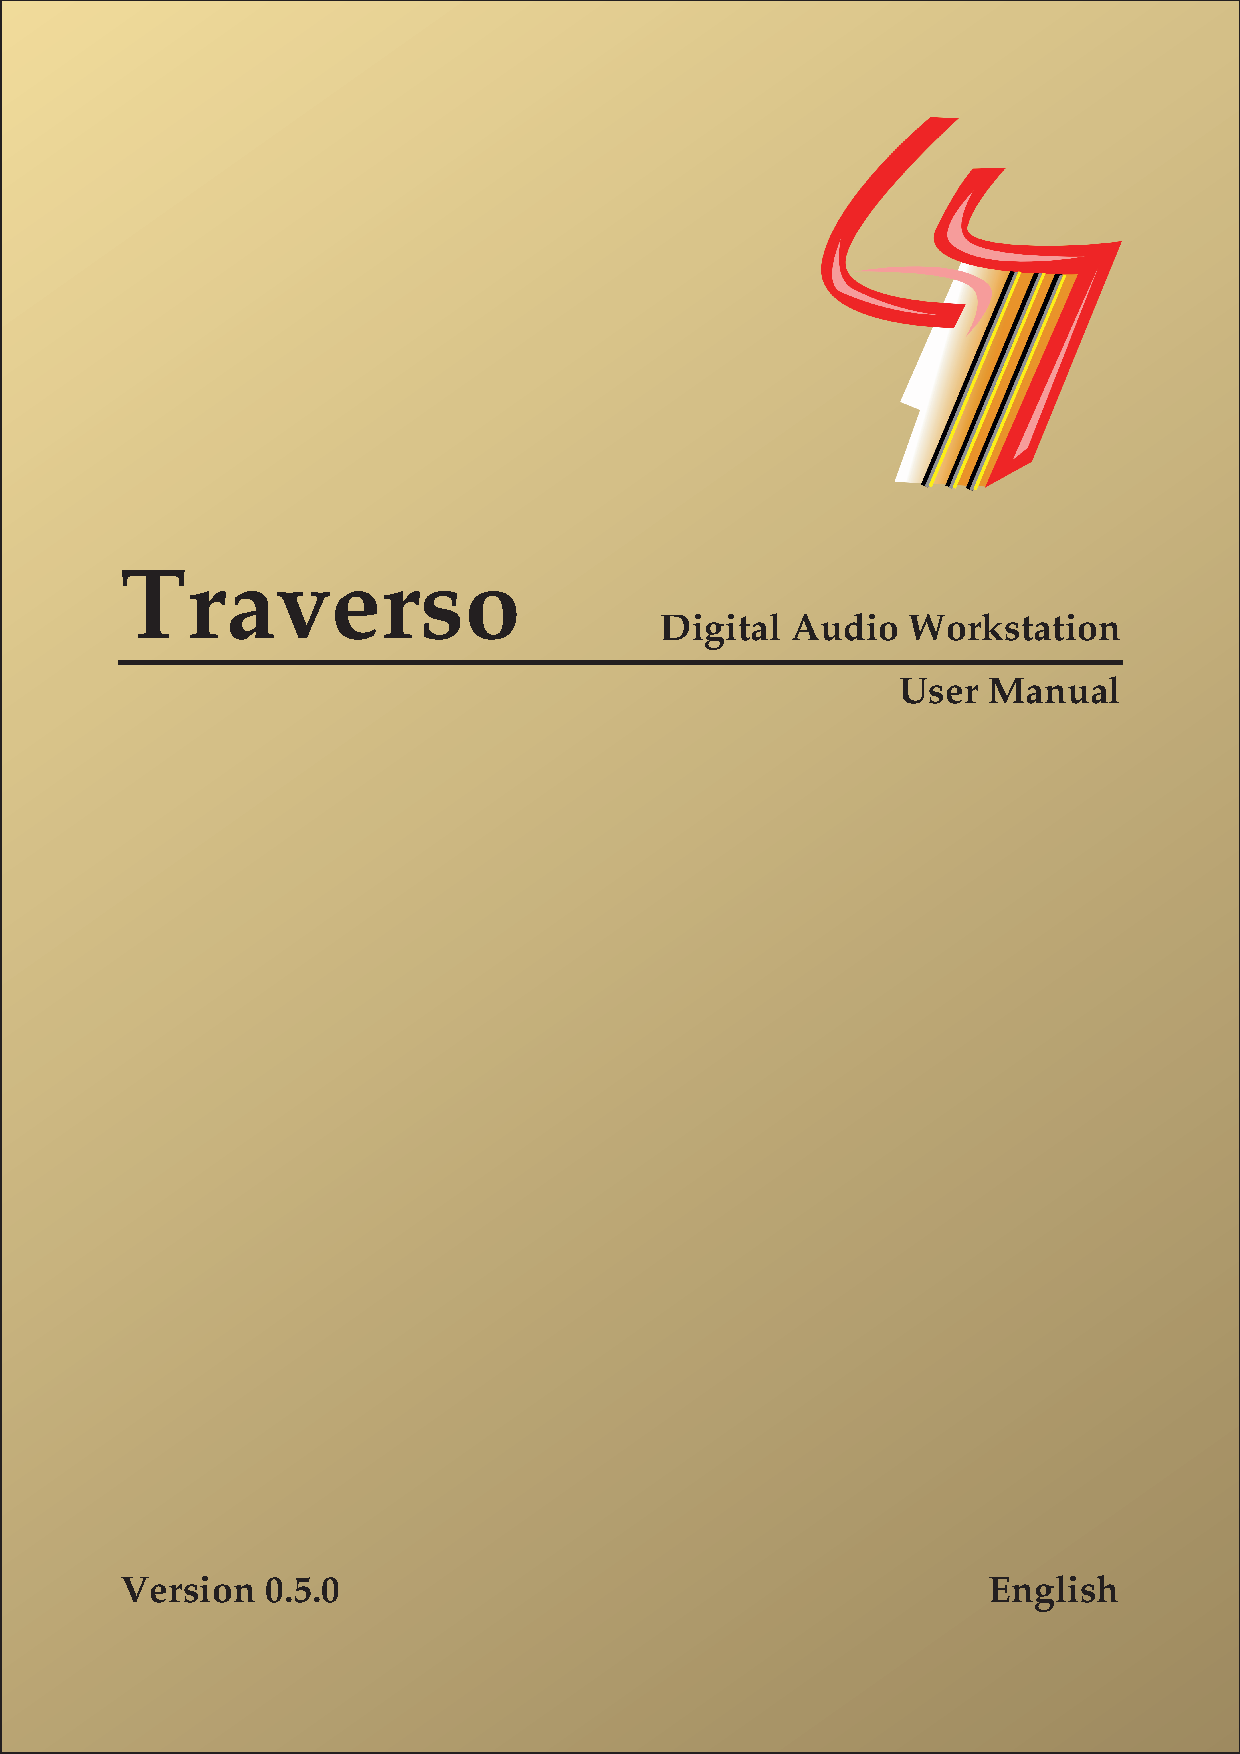
\includepdf{titlepage.pdf}
\end{titlepage}
  \clearemptydoublepage
  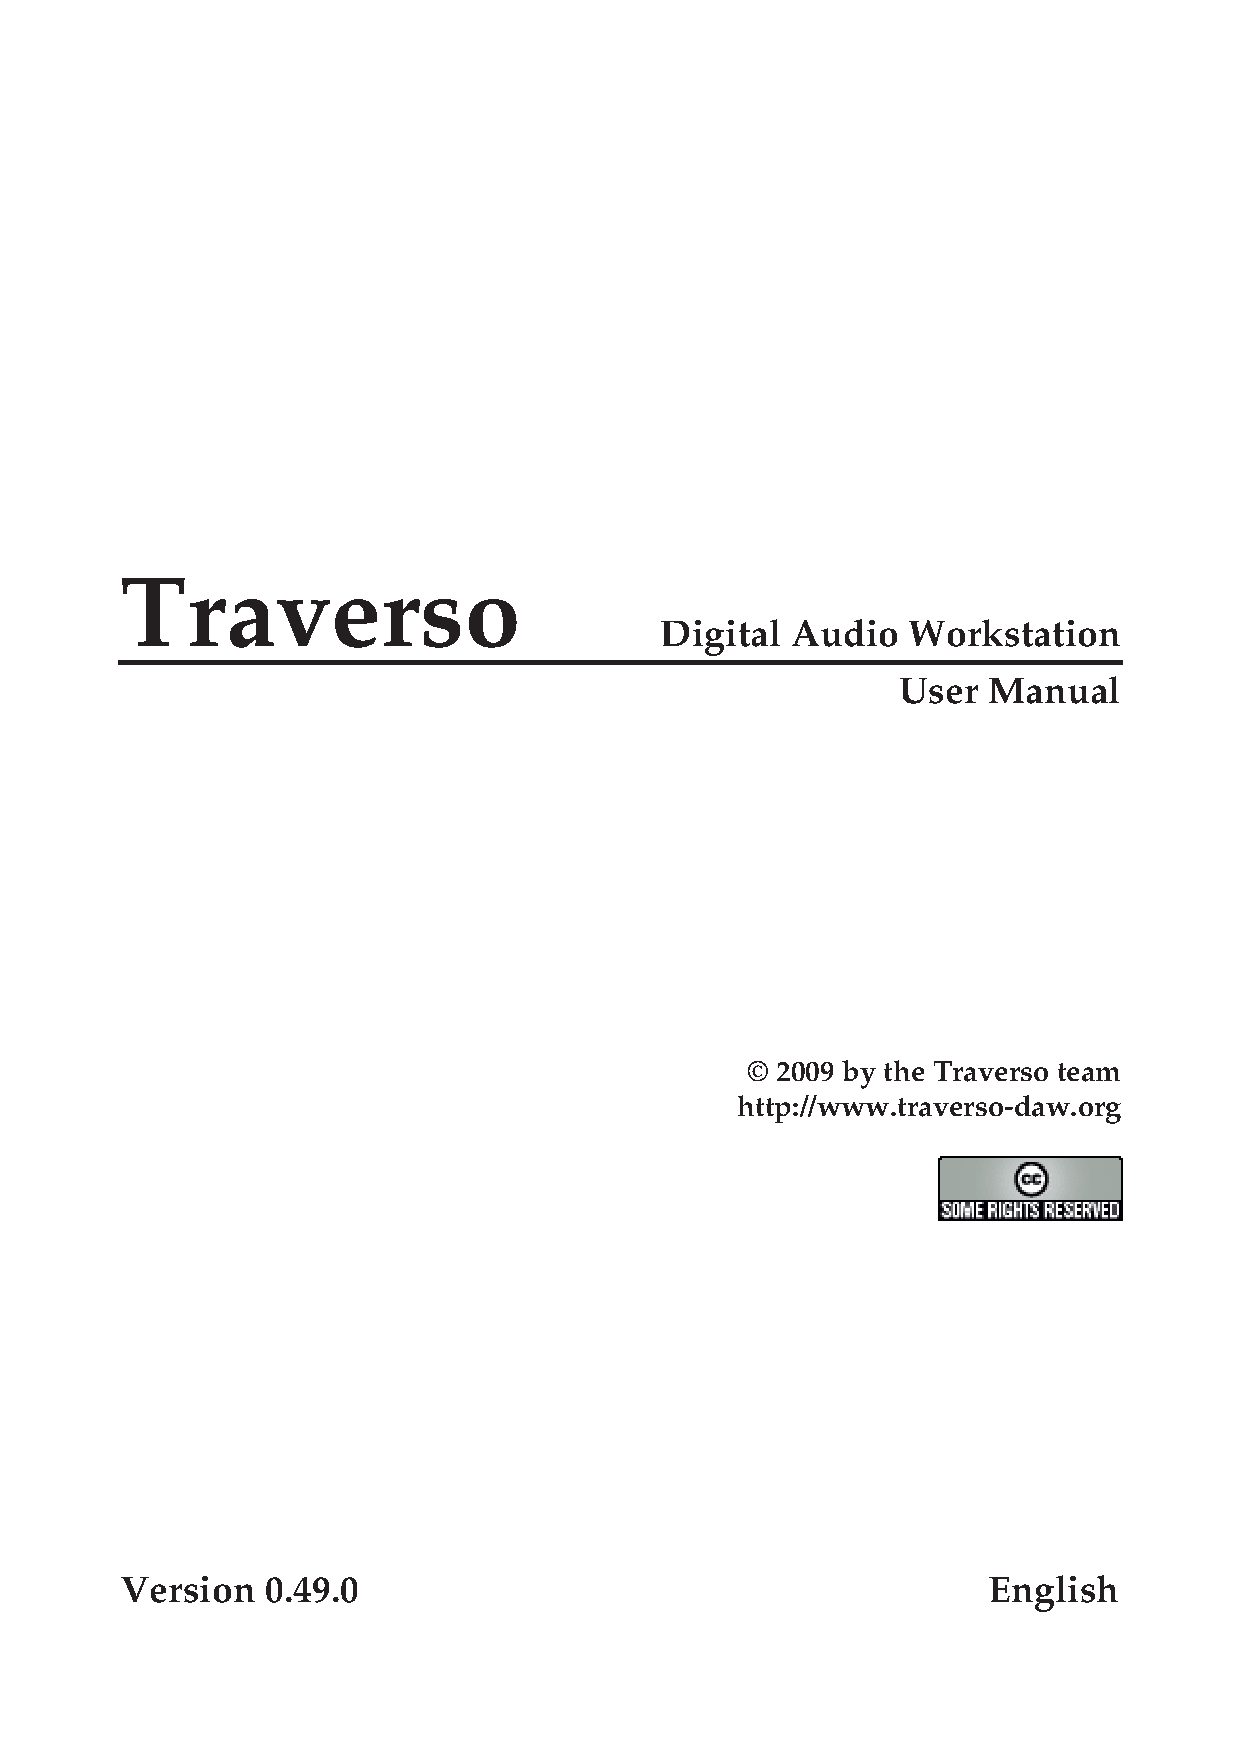
\includepdf{titlepage-author.pdf}
  \clearemptydoublepage

\setcounter{page}{1}
\clearemptydoublepage
\noindent\thispagestyle{empty}
Dieses Dokument steht unter der \emph{Creative Commons Namensnennung-Keine kommerzielle Nutzung 2.5 Niederlande} Lizenz. Um eine Kopie der Lizenz zu erhalten, besuchen sie http://creativecommons.org/licenses/by-nc/2.5/nl/deed.de, oder schreiben sie an Creative Commons, 171 Second Street, Suite 300, San Francisco, California, 94105, USA.\\\\
Zusammengefasst dürfen sie:
  \begin{itemize}
    \item \textbf{Weitergabe} -- das Werk vervielfältigen, verbreiten und öffentlich zugänglich machen
    \item \textbf{Änderungen} -- Bearbeitungen des Werkes anfertigen
  \end{itemize}
  Zu den folgenden Bedingungen:
  \begin{itemize}
    \item \textbf{Namensnennung} Sie müssen den Namen des Autors/Rechteinhabers in der von ihm festgelegten Weise nennen (wodurch aber nicht der Eindruck entstehen darf, Sie oder die Nutzung des Werkes durch Sie würden entlohnt).
    \item \textbf{Keine kommerzielle Nutzung} Dieses Werk darf nicht für kommerzielle Zwecke verwendet werden.
    \item Im Falle einer Verbreitung müssen Sie anderen die Lizenzbedingungen, unter welche dieses Werk fällt, mitteilen. Am einfachsten ist es, einen Link auf die Seite http://creativecommons.org/licenses/by-nc/2.5/nl/deed.de einzubinden.
    \item Jede der vorgenannten Bedingungen kann aufgehoben werden, sofern Sie die Einwilligung des Rechteinhabers dazu erhalten.
    \item Diese Lizenz lässt die Urheberpersönlichkeitsrechte unberührt.
  \end{itemize}
\normalsize


\clearemptydoublepage


\tableofcontents

%--------------- Start of the document --------------

\chapter{Introduction\label{sect_introduction}}
Traverso is a multitrack audio recording and editing program for GNU/Linux with special emphasis on an intuitive, clean, and above all efficient user interface. The program currently supports recording of any number of audio tracks (only limited by hardware capabilities), basic mixing features, and rendering of the  project into various standard audio file formats. The audio engine uses 32 bit floating point precision for all calculations to preserve the highest possible audio quality even after extensive processing.

The user interface uses a contextual interaction concept; instead of relying on the mouse to operate on graphical objects, combinations of mouse and keyboard are used to control the program. This results in a higher flexibility and much faster control of the program when compared to the traditional mouse-based approach. It even goes far beyond the possibilities offered by conventional key shortcuts. The mouse only has to be placed on an object and all functions become available instantly by pressing a key on the keyboard. Since the object under the mouse cursor is automatically selected, this concept is called ``soft selection''.

\section{License}
Traverso is free software; you can redistribute it and/or modify it under the terms of the GNU General Public License as published by the Free Software Foundation; either version 2 of the License, or (at your option) any later version.

This program is distributed in the hope that it will be useful, but WITHOUT ANY WARRANTY; without even the implied warranty of MERCHANTABILITY or FITNESS FOR A PARTICULAR PURPOSE.  See the GNU General Public License for more details.

You should have received a copy of the GNU General Public License along with this program; if not, write to the Free Software Foundation, Inc., 51 Franklin Street, Fifth Floor, Boston, MA  02110-1301, USA.

\section{Motivation}
One of the motivations to introduce the concept of soft selection was our belief in the superiority over the traditional point-and-click concept in regard to efficiency, speed, and ergonomics. The full potential of soft selections develops after an initial learning phase, because something that breaks with existing standards requires time and effort to adopt, and it takes even more time to overcome long-trained habits. But let's have a look at the different working styles with a trivial example. Suppose we want to do something as simple as switching ``Solo'' or ``Mute'' of a track on and off.

\minisec{The ``analogue way''}
In an analogue recording studio with a mixing desk, you have lots of channels, and each channel has lots of buttons, faders, knobs etc. To toggle ``Solo'' or ``Mute'', you identify the channel strip on the mixing desk, and press the corresponding button. If you want to do the same with several channels, you can quickly press many buttons in a row. The fact that there is a dedicated button for each and every function (which is not always trivial to find, depending on the size of the desk), makes it easy to switch the button, but results in mixing desks being huge and complicated electronic devices.

\minisec{The ``Digital Way''}
On a conventional digital audio workstation (DAW) you identify your channel and press the corresponding solo or mute button with the mouse. Depending on the user's skills and the size of the button, this can already be a minor challenge. Switching several channels in a row, however, is very slow and inefficient, because hitting the button requires careful positioning of the mouse cursor each time.

\minisec{The ``Traverso Way'': Soft Selection}
In Traverso you move the mouse over the track you want to process, and press a key on the keyboard, e.g. ``U'' for mute, or ``O'' for solo. Most users hit the key without looking at the keyboard. The track panel is a large area, which is entirely sensitive for the key actions, so even if several tracks should be switched, the mouse cursor can be placed anywhere on the track, requiring much less aiming.

So what is the difference between the digital and the Traverso way? From our experience, moving the mouse on the desk in order to move the cursor on the screen is like using a remote control or a ``finger extension''. It's like being allowed to press buttons on a mixing desk only by using a 30 cm long ruler. One would have to target carefully, and would miss the tiny button most of the time. All in all it would be very tiring and time consuming. Pressing buttons with our fingers, one for mute, one for solo etc., is more ergonomic and intuitive, and we tried to find an interface concept for Traverso which gives a feeling as direct as analogue buttons, without requiring additional hardware control surfaces. So once we have identified the channel we want to process (by hovering the mouse cursor over it), we want a real world button for as many functions as possible. And since our left hand could as well be ready on the keyboard instead of picking our nose, we have all the 104 buttons of our keyboard at our disposal which can give direct access to a large number of actions. This concept is closely related to the handling of action games (e.\,g. ``first-person shooters''), which are highly optimized for efficient and intuitive access to various actions (moving, running, shooting, ducking, \dots) and a large number of tools. To summarize, the advantages of soft selections are:

\begin{itemize}
 \item the distances on the keyboard are shorter than on the screen
 \item the hit-to-miss ratio for key strokes is much better than for buttons on the screen
 \item using both hands allows to work faster and relieves the mouse hand, resulting in a less fatiguing working style
 \item the ``remote control'' feeling is reduced
 \item more actions can be reached directly, requiring less and shallower menu structures
 \item the keys can be found blindly, leading to less distraction from the work flow
\end{itemize}

The downside is a steeper learning curve, particularly at the very beginning, since the keys are not labeled with the function name (``Solo'', ``Mute'', ``Rec'' etc.). But you will soon internalise the commands just as you did with ``Ctrl+C'' for copy and ``Ctrl+V'' for paste. As for the higher efficiency: Could you imagine driving your car, and when approaching a red light first having to open the menu ``brakes'' on your board computer, choose the sub-menu ``change hydraulic pressure'', and adjust the pressure for each wheel manually with the mouse?


\chapter{Installation\label{sect_installation}}
Eine einfache Art Traverso zu installieren ist die Verwendung eines bereitgestellten Installationspakets. Für Traverso \Version\ existieren Binärpakete für einige populäre Linux-Distributionen, sowie Apple OS X auf Intel- und PPC-Architekturen. In der schnelllebigen Opensource-Welt ist es jedoch am einfachsten, sich auf der Traverso-Webseite \cite{trav-hp} über die aktuelle Situation im Bezug auf Installationsmöglichkeiten zu informieren. Alternativ kann man sich das Programm auch aus dem Quellcode kompilieren. Dieser Vorgang wird hier im Detail beschrieben. Traverso wurde erfolgreich auf den Plattformen i586, ia64 und PPC (Linux und OS X) getestet.

\section{Binärpakte}
Vorkompilierte Binärpakete erhält man im Allgemeinen von folgenden Quellen:

\begin{description}
	\item [(K)Ubuntu:] Auf der Download-Seite der Traverso-Webseite \cite{trav-hp} werden Binärpakete für Debian-Derivate bereitgestellt.
	\item [Gentoo:] Traverso ist Teil der offiziellen Distribution. Neue Versionen erscheinen zuerst im Pro-Audio Overlay. Aktuelle Informationen erhält man auf \cite{pro-audio-wiki}.
	\item [SuSE:] Pakete sind auf \cite{suse-ref} erhältlich.
\end{description}

\section{Quellcode kompilieren}
Dieser Abschnitt beschreibt die Übersetzung des Traverso-Quellcodes auf einem (K,X)Ubuntu \Ubuntu\ System. Die Paketnamen können für andere Distributionen etwas abweichen, generell sollte die Anleitung aber leich anzupassen sein. Traverso hängt von der Qt-Bibliothek Version 4.3.1 oder neuer ab.

Zunächst muss das System für die Übersetzung des Quellcodes eingerichtet werden. Wenn wir schon dabei sind, installieren wir noch einige andere nützliche Dinge. Startet also den Paketmanager der Distribution (z.\,B. Synaptic oder Adept) und installiert folgende Pakete:

\begin{itemize}
 \item libqt4-core, libqt4-gui, libqt4-dev
 \item libsndfile1, libsndfile1-dev
 \item libsamplerate0, libsamplerate0-dev
 \item libjack0.100.0-0, libjack0.100.0-dev
 \item libasound2, libasound2-dev
 \item libvorbis, libvorbis-dev, libmad0, libmad0-dev
 \item libwavpack, libwavpack-dev, librdf0, librdf0-dev
 \item libflac++, libflac++-dev, fftw3, fftw3-dev
 \item jackd, qjackctl, gcc, g++, make, cmake
 \item build-essential
 \item libwavpack1, libwavpack-dev, librdf0, librdf0-dev
 \item liblame0$^\bigstar$, liblame-dev$^\bigstar$
 \item libogg0$^\bigstar$, libogg-dev$^\bigstar$
 \item libflac++-dev$^\bigstar$, libflac++6$^\bigstar$
 \item libmad0-dev$^\bigstar$, libmad0$^\bigstar$
\end{itemize}
Auf (K,X)Ubuntu kann auch der folgende Befehl auf einem Terminal eingegeben werden:
\begin{verbatim}
$ sudo apt-get install build-essential libqt4-core \
 libqt4-gui libqt4-dev libsndfile1 libsndfile1-dev \
 libsamplerate0 libsamplerate0-dev libjack0.100.0-0 \
 libjack0.100.0-dev libasound2 libasound2-dev \
 libwavpack1 libwavpack-dev librdf0 librdf0-dev \
 liblame0 liblame-dev \
 libogg0 libogg-dev \
 libflac++-dev libflac++6 \
 libmad0-dev libmad0 \
 fftw3 fftw3-dev jackd qjackctl gcc g++ make cmake
\end{verbatim}

Pakete, die mit $^\bigstar$ markiert sind, sind optional, erweitern aber Traverso um die Unterstützung von komprimierten Dateiformaten wie Ogg/Vorbis, MP3, oder FLAC. Falls sie für die jeweilige Plattform verfügbar sind, empfiehlt es sich auf jeden Fall, sie zu installieren. Für einige Pakete sind evtl. die Universe und Multiverse-Repositorien erforderlich. Weitere Informationen dazu findet man auf den (K,X)Ubuntu-Webseiten, Foren und Wikis.

Falls auf dem gleichen System noch die Qt-Bibliotheken in Version 3 installiert sind, muss eingerichtet werden, dass im folgenden Version 4 verwendet werden soll. Dazu gibt man die folgenden Befehle auf einem Terminal ein, und wählt jeweils die Qt4-Variante aus wenn man gefragt wird:

\begin{verbatim}
$ sudo update-alternatives --config qmake
$ sudo update-alternatives --config moc
$ sudo update-alternatives --config uic
\end{verbatim}

Nun sollte das System in der Lage sein, Traverso zu kompilieren. Ladet euch dazu das aktuelle Quellcode-Archiv von der Traverso-Webseite, und speichert es in eurem Home-Verzeichnis, z.\,B. in /home/deinName/traversosource/. Entpackt und kompiliert wird es mit folgenden Befehlen:

\begin{verbatim}
$ tar -zxvf traverso-x.x.x.tar.gz
$ cd traverso-x.x.x
$ cmake .
$ make -j 2
\end{verbatim}

Dies dauert einige Zeit, und falls das System korrekt eingerichtet wurde, sollte die Übersetzung ohne Fehler durchlaufen. Startet Traverso durch die Eingabe von \texttt{bin/traverso}. Falls das Programm nicht startet, überprüft nochmal ob ihr der Anleitung oben exakt gefolgt seid.

\chapter{Key Actions\label{sect_keyactions}}
Si el ratón está sobre un objeto gráfico, podemos pulsar alguna tecla para realizar una acción. Por ejemplo podemos enmudecer un clip de audio, o modificar la ganancia de una pista. Un comando de teclado es una pulsación simple de tecla, una combinación de teclas, o un movimiento de ratón mientras se mantiene pulsada una tecla. Seguidamente se muestra la notación empleada para las distintas categorías de acciones de teclado, y cómo se ejecutan.

\begin{description}
\item[Acción de teclado sencilla \sact{K} -- Pulsar y soltar:]
Se interpreta como: ``Pulsar y soltar la tecla'', como cuando escribimos una letra.
``K'' es la tecla a usar (\emph{Nota:} Aunque escribimos letras mayúsculas en la notación, simplemente hay que pulsar la tecla ``K'' sin usar nunca las teclas de mayúscula o bloqueo de mayúsculas, a menos que se indique lo contrario). Por ejemplo:
\begin{quotation}
   \sact{F}
\end{quotation}
significa pulse y suelte la tecla ``F''.

\item[Acción de teclado sencilla \hact{K} -- Pulsar y mantener:]
Se interpreta como: ``Pulsar y mantener la tecla''. En un editor de texto, obtendría muchas kkkkkkkkkkk\dots.
Nuevamente, ``K'' es la letra asociada a la acción. Por ejemplo:
\begin{quotation}
   \hact{D}
\end{quotation}
significa presione y mantenga la tecla ``D''.

Por sí mismo, el mantener una tecla pulsada no hace nada. Pero si mueve el ratón mientras una tecla está pulsada, se puede realizar una ``acción analógica''. Por ejemplo mover un clip de audio.

\item[Acción de teclado sencilla \dact{K} -- Pulsar y soltar dos veces:]
Se interpreta como: ``Presione y suelte la tecla dos veces''. Como teclear una letra dos veces, bastante rápido, a la velocidad de un doble click. Por ejemplo:
\begin{quotation}
   \dact{G}
\end{quotation}
significa presionar y soltar la tecla ``G'' dos veces.

\item[Acción de teclado doble \sact{K K} -- Pulsar y soltar:]
Se interpreta como:``Pulse y suelte dos teclas a la vez''. Es una de las acciones más difíciles. Por ejemplo:
\begin{quotation}
   \sact{F G}
\end{quotation}
significa pulsar y soltar las teclas ``F'' y ``G'' a la vez.

\item[Acción de teclado doble \hact{K K} -- Pulsar y mantener:]
Se interpreta como ``Presione y mantenga dos teclas a la vez''. Por ejemplo:
\begin{quotation}
   \hact{F G}
\end{quotation}
significa presionar y mantener las teclas ``F'' y ``G'' a la vez.

Sigue el mismo patrón que la ``Acción de teclado sencilla: pulsar y mantener'', aunque presionando dos teclas. Es un poco más difícil de realizar que con una sola tecla, y en general se reserva para acciones avanzadas.

\item[Acción de teclado doble \dact{K K} -- Pulsar y soltar dos veces:]
Se interpreta como: ``Pulse y suelte ambas teclas dos veces''. Es una acción difícil de ejecutar. Las dos teclas deben pulsarse y soltarse al mismo tiempo, dos veces. y bastante rápido. Por ejemplo:
\begin{quotation}
   \dact{F G}
\end{quotation}
significa pulsar y soltar las teclas ``F'' y ``G'' a la vez, dos veces.

De hecho, este comando no se usa mucho debido a su dificultad de ejecución, pero eso mismo lo convierte en un candidato perfecto para acciones destructivas.
\end{description}

El cursor indica qué tipo de objeto va a recibir la acción de teclado, mostrando una letra cerca del símbolo del cursor. Cuando estamos sobre una pista aparece una T, sobre un clip una C, sobre un fade una F, y sobre un plugin una P (\FigB~\ref{fig_cursor}). Si la acción de teclado no es aplicable al objeto activo, la acción se transmite al objeto que esté debajo. Por ejemplo en el caso de \hact{D} sobre un fade, la acción es enviada al clip de audio en el que está el fade.

Desde el menú ``Ajustes $\rightarrow$ Preferencias\dots'', en la página ``teclado'', pulsando los botones ``Exportar teclado'' o ``Imprimir teclado'', puede exportar el mapa de teclado. Esto permite tener siempre a la vista el mapa de teclado actualizado.

\begin{figure}[htb]
 \centering
 
\includegraphics[height=2\baselineskip]{../images/cursorFloatOverTrack.png}\qquad
 
\includegraphics[height=2\baselineskip]{../images/cursorFloatOverClip.png}\qquad
 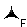
\includegraphics[height=2\baselineskip]{../images/cursorFloatOverFade.png}\qquad
 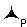
\includegraphics[height=2\baselineskip]{../images/cursorFloatOverPlugin.png}
 \caption{Según el tipo de objeto sobre el que esté el cursor, a su lado aparece una letra diferente. De izquierda a derecha: Pista, Clip, Fade, Plugin.}
 \label{fig_cursor}
\end{figure}

\chapter{Setup\label{sect_setup}}
This chapter assumes that you have Traverso \Version\ or later installed on your system. If not yet so, please refer to chapter \ref{sect_installation} for instructions on how to install the programme.

Start Traverso from the application menu, or by hitting Alt+F2 and entering \texttt{traverso} in the command dialog. The first thing you will see is a file dialog asking you for the project directory. If you don't have one yet, create a new one. This directory will contain all projects, including the audio files. So be aware that if you want to do some serious audio work, you will need \emph{lots} of hard disk space. Change into the directory and press OK. After confirming your selection, the Traverso main window will be shown. It contains different regions which are sensitive for soft selections. The nomenclature used in this manual is shown in \FigT\ \ref{fig_gui01}.

\begin{figure}
 \centering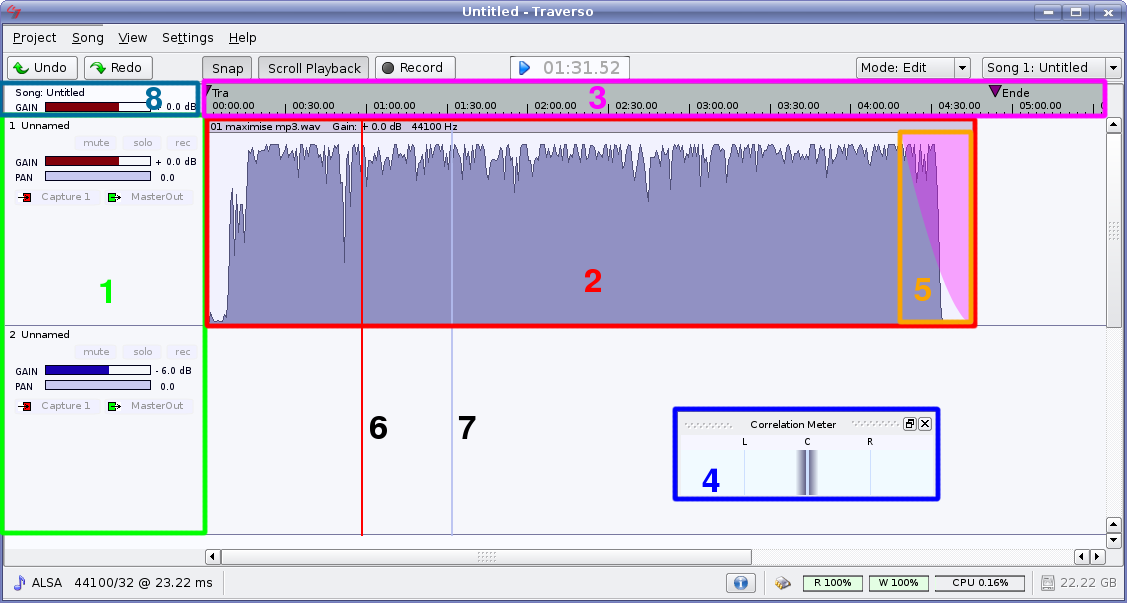
\includegraphics[width=\textwidth]{images/sshot06.png}
 \caption{Interface elements of Traverso: 1 Track panel: If the mouse cursor is hovering over this area, all key actions apply to the track beneath it; 2 Audio clip: Key actions apply to the audio clip; 3 Time line: Key actions apply to markers in the time line; 4 Dock window / Dock widget; 5 Fade out; 6 Work cursor; 7 Play head; 8 Sheet area.}
 \label{fig_gui01}
\end{figure}

Traverso uses dock windows for its tool dialogs, which allows to re-arrange the layout to your own liking. Just grab each one by the title bar and drag it to a new position. You can even stack the dock widgets on top of each other or detach from the main window and move freely. The latter is particularly handy with dual-screen setups, for the main window can occupy one screen, and the dock windows can be moved to the second screen (\FigB\ \ref{fig_mainwin02}).

\begin{figure}
 \centering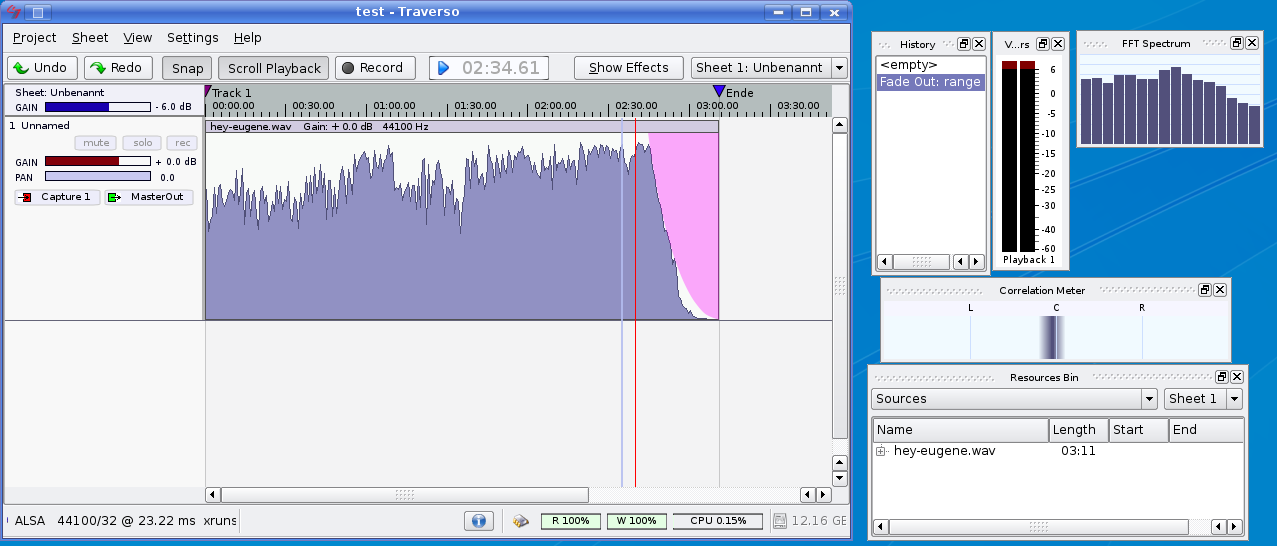
\includegraphics[width=0.9\textwidth]{images/sshot03.png}
 \caption{The dock windows can also be detached from the main window and moved to the second screen in a multi-screen setup.}
 \label{fig_mainwin02}
\end{figure}

\section{The Driver Backend}
Four driver backends are supported to date: The Null driver, ALSA, the jack soundserver, and Port Audio (on Windows and Mac OS X). Let's have a look at all of them, what the advantages and disadvantages are, and how to set them up correctly. The currently loaded driver is displayed in the menu bar.

\subsection{Null Driver}
The Null driver is a fallback solution which is set if no other driver is available, but you won't hear any output as long as the Null Driver is loaded. Hence there's hardly a situation where you want to load it manually. To select a valid driver, click on the \emph{Null Driver} label in the menu bar to open a configuration dialog (\FigB\ \ref{fig_driverconf}).

\subsection{ALSA}
If ALSA is selected, Traverso communicates directly with the ALSA layer, which is only possible if no other application occupies the sound system. So before selecting ALSA as your driver, make sure you stop playback of all other sound applications. Also check the KDE/Gnome system tray for minimized instances of amarok, XMMS, etc. Back in Traverso's driver configuration dialog set the driver to \emph{ALSA}, the rate to 44100, and leave the latency. Then press \emph{Save} and \emph{Apply} and check if the entry in the menu bar has switched to \emph{ALSA}. If it refuses to load the new driver, your sound card may still be occupied by another application, so check again if you correctly stopped all multimedia applications and make sure that the sound daemon (e.\,g. aRTs) shuts down automatically when not used. Then try again to set the driver to ALSA. If it was accepted as a valid driver, the sound driver is set up correctly.

\subsection{Jack}
Traverso can also connect to the jack soundserver, which provides advanced routing features and zero-latency connections between clients. If you don't want to use these features and ALSA works for you, there's no advantage in using jack. We recommend to use \emph{qjackctl}, which allows to easily setup jack for your system. Start the jack daemon by pressing \emph{Start} in qjackctl. When it is running, set the driver in Traverso's configuration dialog (\FigB\ \ref{fig_driverconf}) to \emph{jack} and press \emph{Save} and \emph{Apply}. The menu bar should display \emph{jack} if the driver was loaded correctly. Now go back to qjackctl and open the \emph{Connect} dialog. \emph{Important:} You must set up the connection manually, otherwise you won't hear any sound. Select the Traverso entry in the left part (``Readable Clients''), and alsa\_pcm in the right part (``Writable Clients''), then press \emph{connect}. If a line connecting the two clients is drawn, the sound system is set up correctly.

\begin{figure}
 \centering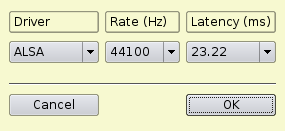
\includegraphics[width=0.5\textwidth]{images/sshot02.png}
 \caption{The audio driver backend can be selected from the menu bar. Traverso supports ALSA, jack, and PortAudio, and has a \emph{Null Driver} as fallback solution if no working driver is available.}
 \label{fig_driverconf}
\end{figure}

\subsection{Port Audio}
Port audio is the only driver backend available on Mac OS X and Microsoft Windows. It connects to the system's native sound system (CoreAudio on OS X, WMME on Windows). Simply select ``PortAudio'' in the driver configuration widget, the samplerate you wish to use, and a latency that works for you.

\section{Recording file format}
From the menu ,,Settings $\rightarrow$ Recording file format'' you can set the file format used for recorded audio. \emph{Wave} has been the standard audio format in the computer world for years. It is uncompressed, and Traverso stores all audio data in 32~bit floating point precision, no matter what bit depth the driver backend was set to. Wave files, however, are limited to a size of 2~GB. For a mono recording in 44100~Hz 32~bit resolution this gives a maximum recording time of approximately 3 hours 20 minutes. For a stereo recording it is only half of that time. If you plan to record longer you should use the \emph{Wave-64} format instead, which can write much larger files. The third format \emph{WavPack} uses a lossless compression algorithm to shrink your files without affecting the quality of the audio data. However, since the encoding is done in real time, more CPU power is required while recording. If you are short of disk space but have a decent CPU, this format is certainly a good choice.

\chapter{Quick Start\label{sect_quickstart}}
The default project automatically created by Traverso contains six empty tracks and is called \emph{Untitled}. So how should we get started?
Let's just start Traverso and import a file to work on.

You will need a wave audio file, or better a couple of them. You can import them from any location on your hard disk, or place them in your Traverso project directory, and further in "Untitled/audiosources" to keep you directories tidy. Back in Traverso, press the I key on an empty track, navigate to the wave files in the file dialog, and select one of them. It will be placed in the track, and after a couple of seconds the wave form will be drawn (it takes a few seconds to calculate the wave form the first time).

We start listening to our imported audio file by pressing the spacebar. The VUMeters will show the level of the output signal. If the VUMeters are not visible, show them from the menu ``Views $\rightarrow$ VUMeters''. Muting the audio clip is done by pressing the U key while the mouse points to the audio clip. To unmute the clip, press U again. To make life easier, throughout this manual we use this notation for pressing the U key: \sact{U}. So, whenever you see a letter enclosed in these brackets, it means press that key once. If you point the cursor to the track background and press \sact{U}, the entire track is muted---and finally the ``mute'' button lights up!

OK, what about splitting our clip into half? Point the mouse to where you want your clip split, and press X, the shorthand notation then will be \sact{X}. All of a sudden we have two clips! Use the undo button in the menu bar to undo the latest action. The clip will return to it's previous state.

Changing the gain of a track or audio clip is done as follows: Point your mouse to the audio clip, and press and hold the G key! The cursor will change to a gain symbol (\FigB\ \ref{fig_gaincursor}). Now move the mouse up/down, and see the gain value change. To make live easier again, the shorthand notation for keys that are pressed \emph{and} held is \hact{G}. When releasing the G key, the cursor returns to it's normal state, and the new gain value will be used. If you point the cursor to the background of the track, e.\,g. between two clips or to the track panel on the left (where the ``Solo'', ``Mute'', and ``Rec'' buttons are), holding \hact{G} and moving the mouse will change the gain of the entire track. Instead of moving the mouse, try scrolling with the mouse wheel while holding \hact{G} to change the gain in very small steps. These actions, as you can see in the History view, are also un/redoable. You can also select an entry in the history view to jump directly to a certain state in the history.

\begin{figure}
 \centering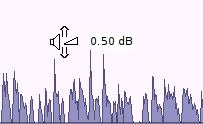
\includegraphics[width=0.4\textwidth]{images/gain-cursor.png}
 \caption{The cursor changes to a gain symbol during the \hact{G} action.}
 \label{fig_gaincursor}
\end{figure}

Up to now we used some simple and easily memorable actions, but there are of course a lot more. But how to know which functions are available for a track or audio clip? Fortunately, there are menus available. You can either use the righ mouse button to popup the menu for the object beneath the mouse cursor, or use \sact{Q} (by now you know that this means pressing the Q key). The menu shows the available functions, and how to perform them on the keyboard (\FigB\ \ref{fig_clipmenu})!

\begin{figure}
 \centering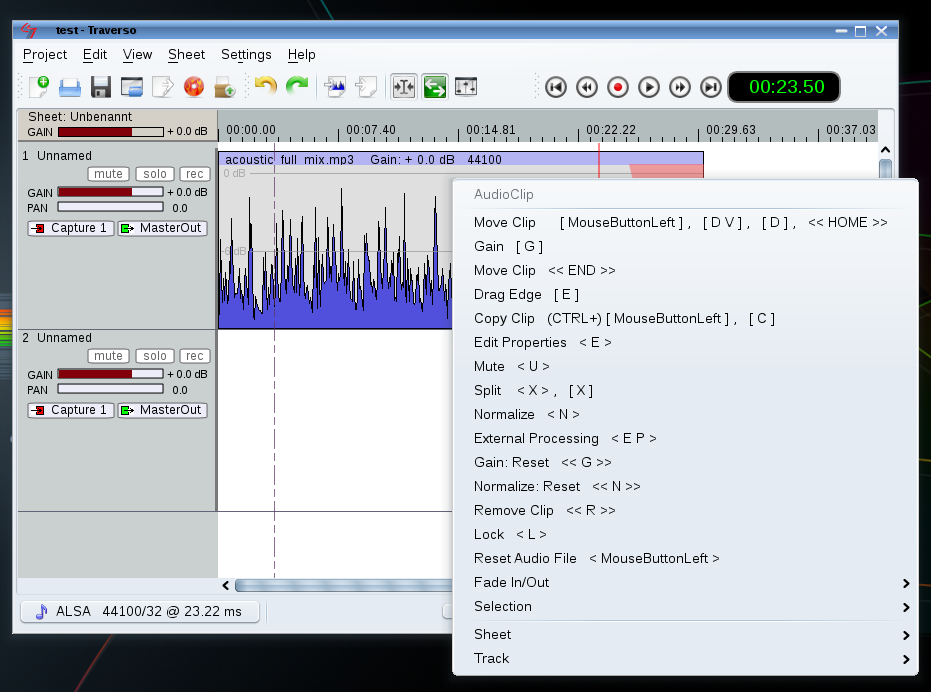
\includegraphics[width=\textwidth]{images/clipmenu.png}
 \caption{Pressing \sact{Q} or the right mouse button on an audio clip shows a menu with all available actions.}
 \label{fig_clipmenu}
\end{figure}

Moving the audio clip can be done by pressing the left mouse button, and keeping it pressed, or by doing the same with the D key. According to our notation scheme that would be \hact{D} or \hact{Left MouseButton}. Alternatively, you can just drag the audio clip with the mousecursor. You can move the mouse freely to position the audio clip to your own liking, the view will automatically scroll if the mouse comes close to the boundaries of the view. Also check out the \hact{Z} and \hact{S} actions to zoom and move the horizontal slider.

By now we learned two kinds of actions, the single key actions \sact{K}, and the hold actions \hact{K}. We also learned that key actions always work on the object beneath the mouse cursor. But before you start exploring the possibilities of Traverso on your own, let's look at some more (randomly selected) functions.

If you want to reset the gain of an audio clip or track to 0 dB, point the mouse cursor to a clip and press the G key twice. This works just like double-clicking with the mouse. In our notation scheme, a double key stroke is notated as \dact{G}. You will see that this action first resets the gain to 0 dB, and if called again, toggles the gain between $-6$ and 0 dB. This also works on the track gain.

As a last example let's delete an audio clip. First select the clip by hitting \sact{S} on it. Its background will become dark. Then hit X and C twice at the same time. This action is difficult to perform, maybe you need a couple of attempts to get it right. But this makes the action ideal for ``dangerous'' function which should by no means happen accidentally. According to our notation scheme this function writes as \dact{X C}. An overview of all available action types is given in chapter \ref{sect_keyactions}. Chapters \ref{sect_recording} and \ref{sect_mixing} provide more detailed information on recording and mixing.


\chapter{Recording\label{sect_recording}}
\section{Creating a new project}
To make some test recordings we first create a new project. Start Traverso and select ``New\dots''. Enter a name, set the number of sheets to 1, the number of tracks to 2, and leave the rest empty. Then press ``OK'' to create the project and show it's first sheet. Note: All recorded audio data will be stored in \texttt{project\_dir/project\_name/audiosources}, so if you followed our advice and selected a project directory on a partition with lots of free space, you shouldn't run out of disk space now.

\section{Setting up the driver}
To set up the driver backend, open the preferences dialog by clicking ``Settings $\rightarrow$ Preferences\dots'' (\FigB\ \ref{fig_driversettings}). Which driver is appropriate for your system is described in chapter \ref{sect_setup}. In the driver configuration one can choose the sampling rate, and Traverso always uses the sampling rate of the driver backend for its recordings. Traverso's audio engine works entirely in 32 bit floating point precision, and you can chose from the menu ``Settings $\rightarrow$ Recording file format'' whether the data should be stored in a standard Wave format, in Wave-64, or in WavPack. The bit resolution will always be 32~bit floating point.

\begin{figure}
 \centering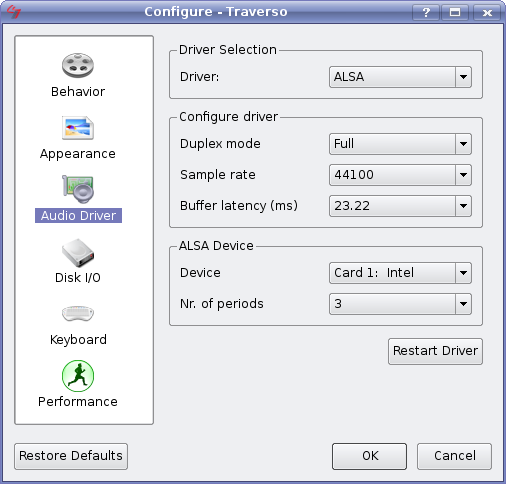
\includegraphics[width=0.7\textwidth]{images/driversettings.png}
 \caption{In ``Settings $\rightarrow$ Preferences\dots'', all driver related parameters can be set.}
 \label{fig_driversettings}
\end{figure}

\section{Recording}
Make sure a sound source is connected to the line-in bus of your sound card, and also make sure it really is playing back. In Traverso hit \sact{B} on the first track and select ``Capture 1'' as input bus, then hit \sact{A} to arm the first track. As soon as the track is armed, you should see the VUMeter indicating an input signal on Capture1. If not, the problem is most probably to be searched outside of Traverso. If you are sure your cable connections are correct, open KMix or a similar mixer applet to configure your sound card. As shown in \FigT\ \ref{fig_kmix01}, the Line and Capture channels had to be armed and un-muted on our test system before the line-in signal got through to Traverso.

\begin{figure}
 \centering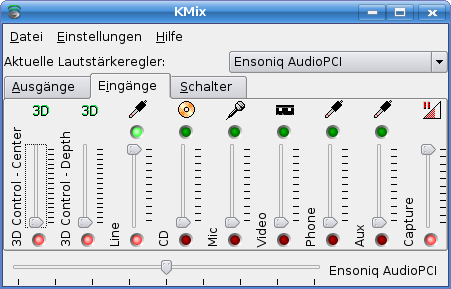
\includegraphics[width=0.75\textwidth]{images/kmix01.png}
 \caption{KMix can be used to configure the sound card. Make sure the correct input channels (Line and Capture) are un-muted and set for recording (green and red buttons).}
 \label{fig_kmix01}
\end{figure}

When you are ready to record, press the \texttt{Record} button in the title bar or hit CTRL+\sact{SPACE} to start the recording, and hit \sact{SPACE} to stop recording. That's it. In order to rehearse the recording, place the work cursor before the newly recorded clips, and press \sact{SPACE} to start playback. Once you have finished recording a track, don't forget to unarm it by pressing \sact{A}, or unarm all armed tracks at once by hitting \dact{A}.


\chapter{Mixing\label{sect_mixing}}
Mixing features in Traverso \Version\ currently include gain, panorama, different fade shapes for fade-in and -out, trimming, splitting, moving of audio clips, and gain curves. An infrastructure for effect plugins using the LV2 standard is implemented, but  the LV2 standard and plugins are still under heavy construction. Traverso also has basic support for using Sox to process audio clips.

\section{Moving, trimming, splitting}
Clips can be moved freely by holding \hact{D} and moving the mouse. If snapping is active (\sact{S~N}), both ends of the dragged clip will snap to the beginning of the sheet, edges of other clips, markers, and to the work cursor.

Move the mouse cursor on a clip, hold \hact{E}, and move the mouse horizontally to drag the edge of the clip which is nearest to the mouse position. If snapping is active, the edge will snap to the positions described above.

Audio clips can be split by pointing the mouse cursor to the desired position and pressing \sact{X}. Of course the edges of the two clip fragments can be fine-tuned by holding \hact{E} as describes above.

\section{Fades}
Both ends of a clip can be faded smoothly by holding \hact{F} on the left or right half of the clip and moving the mouse horizontally. On the left half the key action refers to the fade-in, on the right half it refers to the fade-out. Several fade shapes are available, which can be toggled by \sact{M} (\FigB~\ref{fig_fades01}).

\begin{figure}[t]
 \centering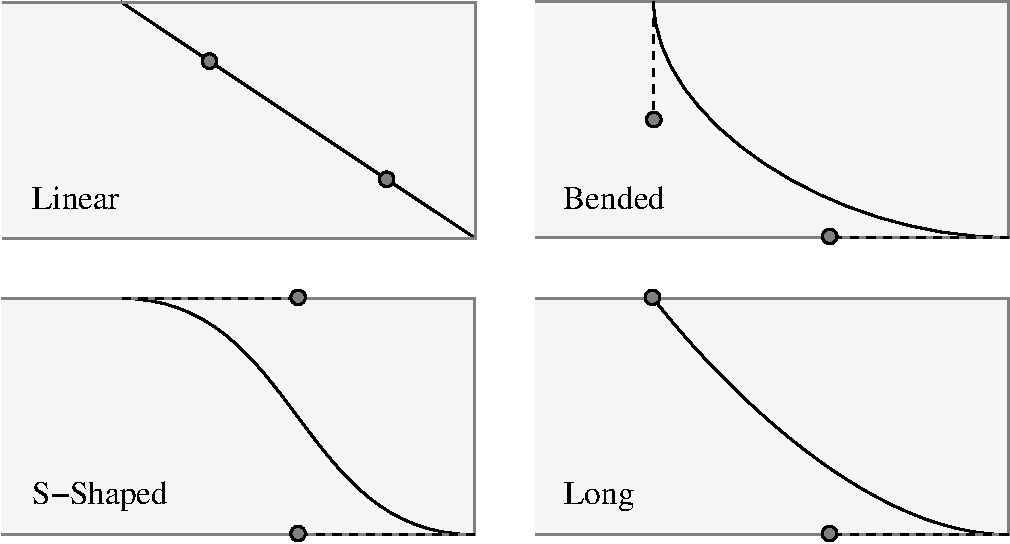
\includegraphics[width=0.8\textwidth]{../images/fades}
 \caption{Different fade shapes are available in Traverso. Fade curves are defined as splines with two control points (circles) which can be modified by the values ``bending'' and ``strength''.}
 \label{fig_fades01}
\end{figure}

All shapes are based on a cubic spline curve with four knots. Two knots define the bending of the non-linear shapes. The positions of these control knots can be modified by two values ``bending'' and ``strength''. ``Bending'' defines the direction of the tangent in the end point, whereas ``strength'' changes the weight of the tangent (\FigB~\ref{fig_fades02}). It is not possible to move the control knots freely and independently, instead Traverso knows several modes which are relevant for fade shapes (\FigB~\ref{fig_fades01}):

\begin{figure}[t]
 \centering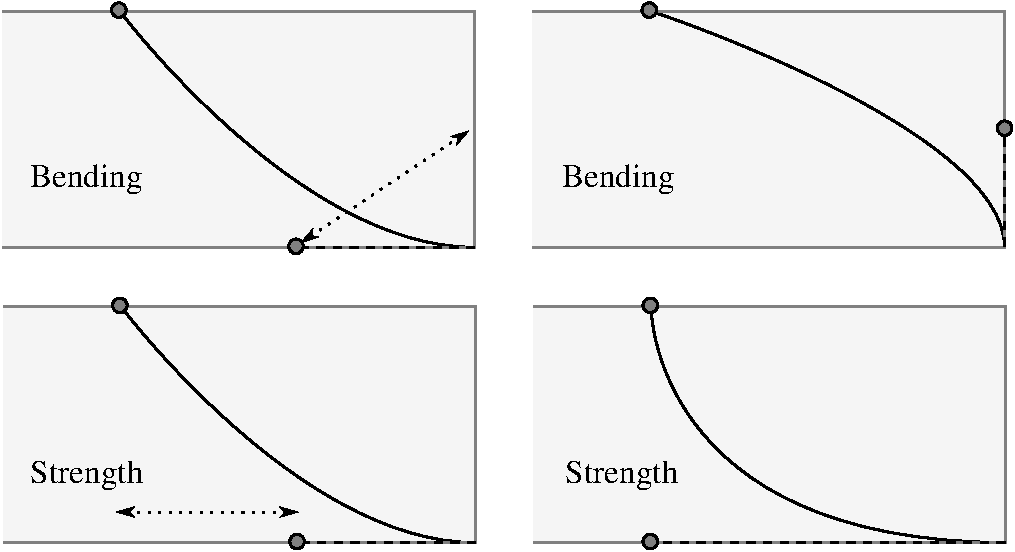
\includegraphics[width=0.8\textwidth]{../images/fades2}
 \caption{Bending and strength values can be used to alter the shape of the fade curves. (Demonstrated with the ``Long'' mode.)}
 \label{fig_fades02}
\end{figure}

\subsection{Linear}
Linear fades are a straight line between the start and end point. The control knots can't be changed. Linear fades tend to sound rather abrupt at the low-level end of the fade, and are thus not the preferred mode for long fade-outs, e.\,g. at the end of a sheet.

\subsection{S-shaped}
The S-shaped mode starts with a horizontal tangent, is steep a the center, and passes into a horizontal tangent again. The beginning and end are very smooth, but the center part can sometimes change too quickly in short S-fades. The ``strength'' parameter can be used to soften the center part and make the volume change less obvious. The ``bending'' factor should usually remain between linear and horizontal tangents, however, vertical tangents can be used for effects.

\subsection{Bended}
The bended mode acts similar to the S-shaped mode, but the control knots point to the same side. This mode can be used to achieve a very fast volume drop at the beginning of the fade-out, and very soft towards the end. Both control parameters are useful to find the best balance between a beginning that is not too fast, and an ending that is still slow enough for a soft fade-out effect.

\subsection{Long}
The long mode only allows to change the control knot at the low-level end of the fade. This mode is often used for very smooth fade-outs, e.\,g. at the end of a sheet. The high-level end changes fastly, but the low-level tail is very soft. The long mode often sounds more musical than a similar bended mode.

The fades can be edited numerically by pressing \sact{E} on a clip, and changing to the page ``Fades'' in the clip settings dialog.

\section{Gain curve}
Gain curves are a powerful feature to change the gain of an audio clip in the time line. The curves are child elements of audio clips, therefore their \emph{relative} position to the audio clip will always stays the same. To change to effects mode, select the entry ``Mode: Effects'' from the dropdown menu in the menu bar (\FigB~\ref{fig_gcurve01}). To change back to edit mode ``Mode: Edit''. A default curve node is added automatically at the beginning of the clip at 0~dB. Additional nodes can be created by \dact{C} at the position of the mouse cursor. Nodes can also be dragged (\hact{D}) and removed (\dact{R}). These actions always apply to the node closest to the mouse cursor, which is indicated by a different colour.

\begin{figure}[t]
 \centering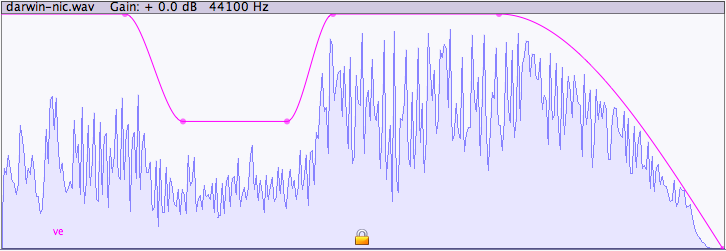
\includegraphics[width=\textwidth]{../images/gcurve01}
 \caption{The ``effects mode'' of Traverso can be activated from the dropdown menu in the menu bar. Gain curves are only visible in that mode. Nodes can be added, removed, and dragged freely.}
 \label{fig_gcurve01}
\end{figure}

\section{Plugins}
Traverso supports the LV2 plugin interface, which is the successor of the LADSPA standard. Plugins can be added to tracks by pressing \sact{F5}, which opens a list of all LV2 plugins installed on the system (\FigB~\ref{fig_pluglist}). Active plugins will be shown as semi-transparent fields in the track view. These fields have their own context menu; just try it out by holding the mouse on them and pressing \sact{Q} or \sact{Right Mouse Button}. Pressing \sact{E} will open a generic dialog, which allows to adjust the plugin parameters. Plugins can also be bypassed (\sact{B}) and removed (\dact{R}). Version 0.40.x inserts all plugins post-fader. More flexible solutions will follow in upcoming versions.

\begin{figure}[t]
 \centering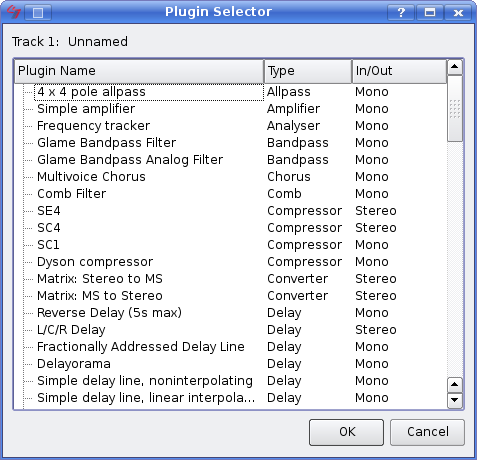
\includegraphics[width=0.6\textwidth]{../images/plugin-list}
 \caption{Plugins can be added to a track by pressing \sact{F5}.}
 \label{fig_pluglist}
\end{figure}



\chapter{Laying out a CD\label{sect_cdburning}}
\section{Requirements}
This chapter describes how to arrange and write a Red Book compatible audio CD. Traverso uses \texttt{cdrdao} to actually write the CD, so this program must be installed on the system. \texttt{cdrdao} is available from the official repositories of all  major and up-to-date Linux distributions, it is thus recommended to install it via the distribution's package manager. The Windows and Mac OS X installer takes care of installing cdrdao for you, so if you are on one of these platforms, you skip this section!

\footnotesize
\begin{verbatim}
tux@linux:~$ cdrdao

Cdrdao version 1.2.2 - (C) Andreas Mueller <andreas@daneb.de>
  SCSI interface library - (C) Joerg Schilling
  Paranoia DAE library - (C) Monty

Check http://cdrdao.sourceforge.net/drives.html#dt for current 
driver tables.


Usage: cdrdao <command> [options] [toc-file]
command:
...
\end{verbatim}
\normalsize

If the command was not found, the next section explains how to install \texttt{cdrdao} on the Linux platform.

\subsection{Linux}
Installing \texttt{cdrdao} on Linux is straight forward, since it is part of all major distributions. Use your distribution's package manager (e.\,g. Synaptic or Adept on (K)Ubuntu, Yast on SuSE), search for \texttt{cdrdao} and install the binary package. Alternatively, you can install it from a terminal. The commands will differ depending on the distribution. For (K,X)Ubuntu, enter the following lines in a terminal:

\begin{verbatim}
sudo apt-get update
sudo apt-get install cdrdao
\end{verbatim}


\section{Tracks and Markers}
There are basically two ways of defining tracks for a CD. Each sheet can be a track, or the entire CD can be arranged in the timeline of a sheet and tracks are defined by markers. Combinations of the two ways are also possible. Let's have a closer look at these two concepts.

\subsection{A Sheet is a CD-Track}
As you may have noticed, Traverso allows to have several sheets in a project. Some people like this feature, as one can combine all sheets of an album in one project, and still focus on one sheet at a time. If you want to write a CD containing all sheets of your project, make sure you check the ``All sheets'' button in the export dialogue. Each sheet will be rendered to a track, from position 00:00:00 up to the end of the last audio clip, and consequently each sheet will become a track on the CD.

\subsection{CD in a timeline}
Sometimes it is important to fine-tune the transition from one track to the next, e.\,g. by adding a little bit of silence in between, or by fading the previous track into the next one. In that case it can be easier to arrange the entire CD in one timeline and split it into tracks using markers. Let's look at an example in order to show how this works. (Look at \FigT~\ref{fig_markers01} if you get lost with the explanations.) Open or create a project with only two audio clips. Suppose we want clip 1 to be track 1 on the CD, and clip 2 will be track 2. Position them on the first and maybe second track, starting at position 00:00:00, as you want to hear them on the CD. Leave some silence between the end of clip 1 and the beginning of clip 2. To get Traverso to start a new CD track there, position the mouse cursor on the gap between the two clips, and press \sact{M}. This adds a small triangle to the timeline at the position of the mouse cursor, and two more at position 00:00:00 and at the end of clip 2. The latter one is labelled ``End'', and it marks the end of the CD. You can shift it a bit further back if you don't want the CD to stop right there (remember you  can have reverb tails extending beyond the last audio sample, which you don't want to cut off).

\begin{figure}[t]
 \centering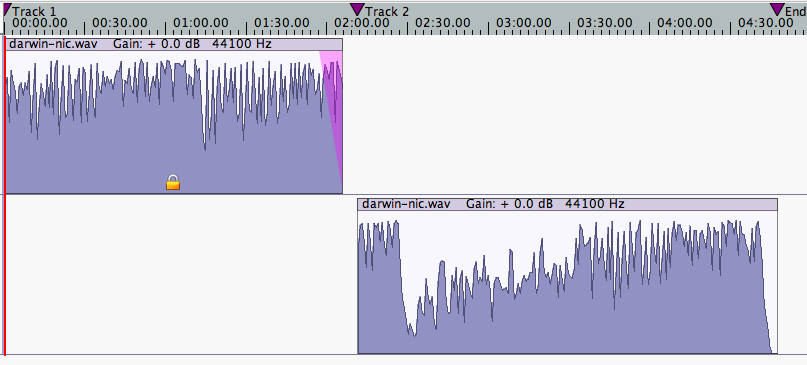
\includegraphics[width=\textwidth]{../images/markers01}
 \caption{If a CD is arranged in one sheet, markers can be used to define CD tracks. Always keep the ones at position 00:00:00 and at the end.}
 \label{fig_markers01}
\end{figure}

These triangles are CD track markers, and they can be moved, added, and deleted freely (press \sact{Q} on the timeline to list all available functions.) However, it is also possible to create setups which don't make sense. E.\,g. only having one track marker in the timeline. In such cases, Traverso tries to guess the most sensible solution, and adds markers on the fly at positions it considers appropriate (which is usually at position 00:00:00 and after the last sample of the sheet containing audio data). Traverso also supports CD-text, which can be entered in the marker dialogue ``Sheet $\rightarrow$ Marker Editor\dots'' (\FigB~\ref{fig_marker-editor}). It is also possible to export the table of contents of the CD as an HTML file from this dialog. Album-wide CD-text can be entered in the project settings, opened from ``Project $\rightarrow$ Manage Project'', in the tab ``CD Text''.

\begin{figure}[ht]
 \centering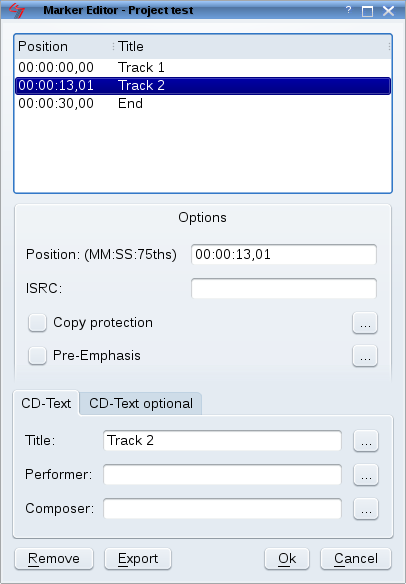
\includegraphics[width=0.6\textwidth]{../images/marker-editor}
 \caption{The marker dialogue opened from ``Sheet $\rightarrow$ Marker Editor\dots'' allows to add CD-text, modify the markers, and export the table of contents as an HTML file.}
 \label{fig_marker-editor}
\end{figure}

Once the CD is laid out to your satisfaction, press \sact{F8} or go to ``Project $\rightarrow$ CD writing\dots'' to open the CD writing dialogue (\FigB~\ref{fig_exportdlg}). Now you must decide if you want to burn the current sheet (using markers to define CD tracks), or the entire project (each sheet becomes a track). If you check ``Export to disk only'', no CD will be written, but only a *.toc file and *.wav files for \texttt{cdrdao}.

In order to export the sheet or project to the hard disk, press \sact{F9} or select ``Project $\rightarrow$ Export\dots'' from the menu. This opens another dialogue (\FigB~\ref{fig_exportdlg}), where you can select a file format and adjust various parameters. Traverso supports most of the common and popular file formats, including Wave, AIFF, FLAC, WavPack, Ogg Vorbis, and MP3. If one or more file formats are not available on your system, Traverso was probably compiled without support for it. Some distributors prefer not to include support for certain compressed formats due to legal reasons. In that case you either have to live with it, or you have to compile Traverso yourself with support for the required codec.

Note for OS X users: CD writing support is still experimental. You can choose between several burning devices: IODVDServices, IODVDServices/2, IOCompactDiscServices, IOCompactDiscServices/2. These are hard-coded, so you probably don't have all of them installed. IOCompactDiscServices should only be used for old drives without DVD reading support. If you have multiple DVD drives, use IODVDServices or IODVDServices/2 to access the first and the second drive. In most cases IODVDServices will be the only working solution.

\begin{figure}[t]
 \centering
 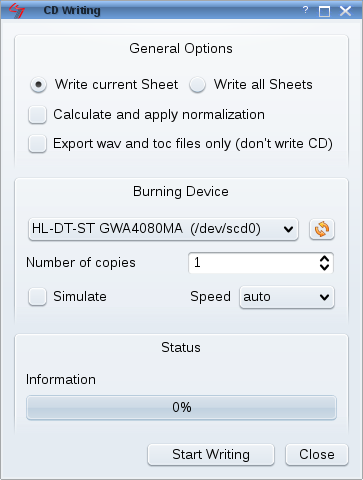
\includegraphics[width=0.4\textwidth]{../images/exportdlg}\qquad
 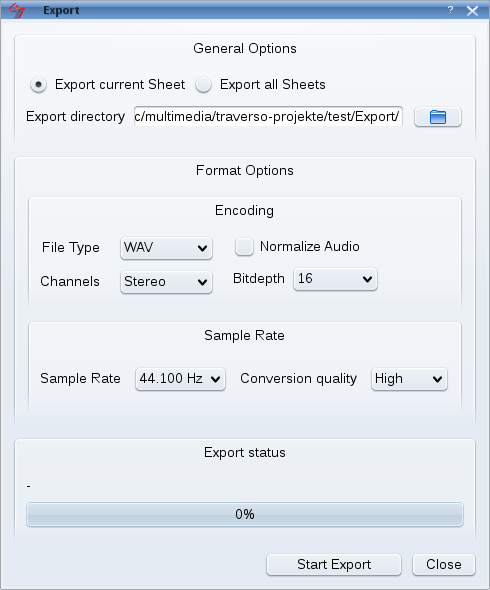
\includegraphics[width=0.5\textwidth]{../images/exportdlg1}
 \caption{\sact{F8} opens a dialogue that allows to burn the current sheet or the entire project on a CD (left). \sact{F9} opens an export dialogue which writes the current sheet or the entire project to the hard disk (right).}
 \label{fig_exportdlg}
\end{figure}


\chapter{Tools\label{sect_tools}}
\section{Korrelationsgradanzeige}
Die Korrelationsgradanzeige in Traverso analysiert den linken und rechten Kanal des Masterausgangs, und berechnet deren Korrelationskoeffizienten. Im Gegensatz zu vielen anderen Programmen interpretiert sie den Wert als Ma"s für die Stereobreite des Signals, und stellt den Wert entsprechend dar.

Um zu erklären wozu man die Korrelation überwachen muss nehmen wir an, eine reine Sinuswelle gleicher Frequenz wird sowohl über den rechten als auch über den linken Kanal abgespielt. Werden die beiden Wellen addiert (dies geschieht, wenn das Signal Mono-geschaltet wird, oder wenn sich die Signale in der Luft überlagern), so entsteht ein Summensignal, das je nach Phasenunterschied der beiden Wellen Interferenzerscheinungen aufweist. Das hei"st, wenn zwei positive Werte addiert werden, entsteht ein grö"serer Wert, aber wenn ein positiver und ein negativer Wert summiert werden, entsteht ein Wert mit kleinerem Betrag als die Beträge der Summanden. In einigen Fällen kann dies sogar zu kompletter Auslöschung des Signals führen (\FigB\ \ref{fig_interference}).

\begin{figure}
	\centering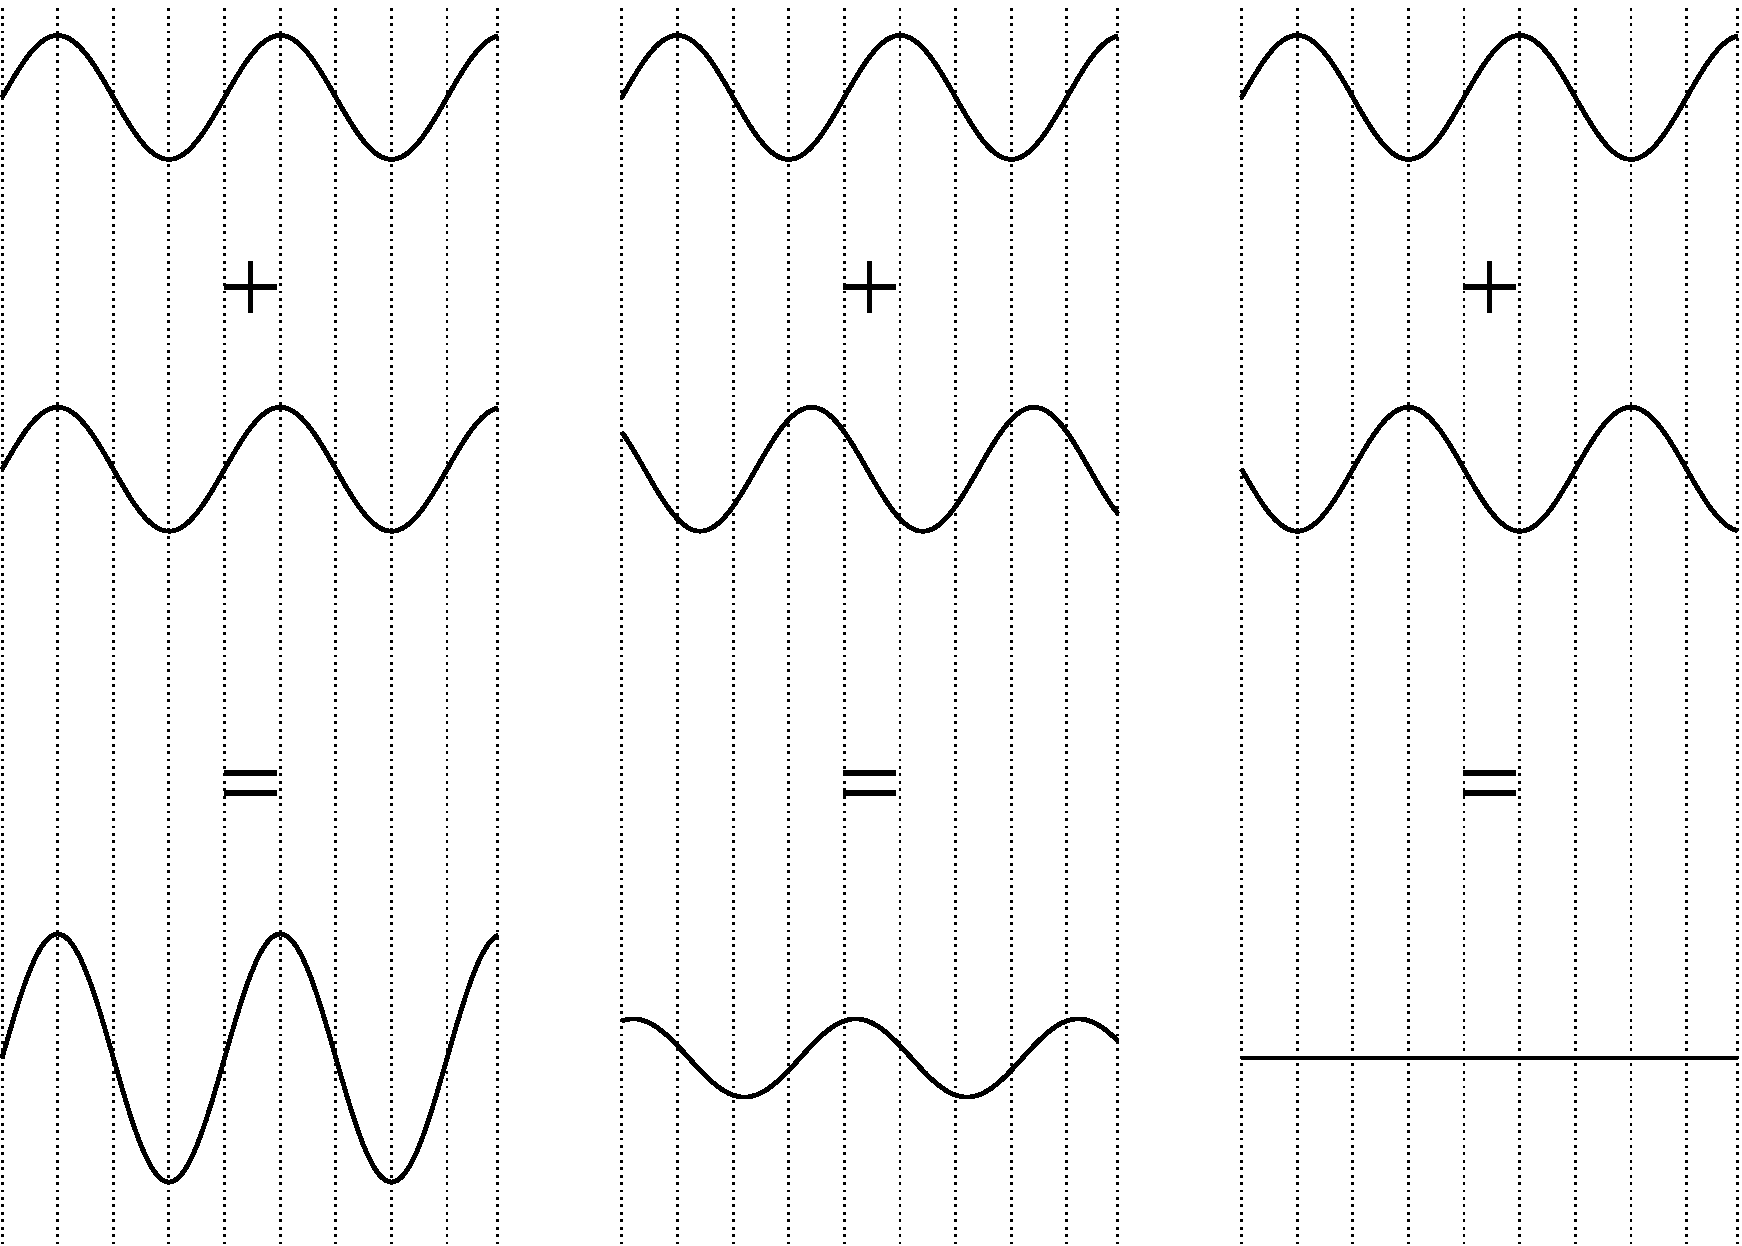
\includegraphics[width=0.8\textwidth]{images/sine01}
	\caption{Werden zwei Sinuswellen addiert, entstehen Interferenzen die entweder zu einer Verstärkung (in Phase, links), einem mehr oder weniger unveränderten Signal (unkorreliert, mitte), oder zu Auslöschung führen können (au"ser Phase, rechts).}
	\label{fig_interference}
\end{figure}

Enthalten die beiden Kanäle komplexere Audiodaten, zum Beispiel Musik oder Sprache, wirken solche Auslöschungen nicht auf das ganze Signal, sondern nur auf gewisse Frequenzbereiche. Der Klang wird dadurch ,,hohl'' oder anderweitig verändert. Solche Effekte sind natürlich in keiner qualitativ hochwertigen Produktion akzeptabel. Normalerweise können sie leicht durch Probehören identifiziert werden, doch bieten heutzutage Analyseprogramme visuelle Darstellungen von Audiosignalen auf vielfältige Weise, was als gro"ser Vorteil gegenüber analogen Lösungen gewertet wird. Es gibt unterschiedliche Arten der Darstellung von Korrelationskoeffizienten. Um zu verstehen, wie die Korrelationsgrad-Darstellung in Traverso zustande kommt und zu interpretieren ist, müssen wir die Berechnung noch etwas genauer betrachten.

Der Grad der Korrelation wird grundsätzlich über den \emph{linearen Korrelationskoeffizienten} $r$ bestimmt, der über eine Reihe von Wertepaaren $(x_i,y_i)$ berechnet wird:
\[
r = \frac{\sum\limits_{i}(x_i - \bar{x})(y_i - \bar{y})}{\sqrt{\sum\limits_{i}(x_i - \bar{x})^2} \sqrt{\sum\limits_{i}(y_i - \bar{y})^2}}
\]
$r$ reicht von $-1.0$ bis $1.0$. Ein Wert von $r = 1.0$ bedeutet, dass das linke und rechte Signal perfekt korrelieren. Das Mastersignal wäre mono in diesem Fall, da es keine Phasendifferenz zwischen dem linken und rechten Signal gibt. Je mehr Unterschiede es gibt, desto tiefer wird der Korrelationskoeffizient. Bei vollkommen unkorrelierten Signalen wird $r = 0.0$. Dies bedeutet, dass es keinerlei Ähnlichkeit zwischen dem linken und rechten Signal gibt. Solch ein Signal produziert ein weites Stereobild, jedoch ohne Gefahr von Phasenauslöschungen. Erst wenn man die Unterschiede der beiden Signale weiter ,,vergrö"sert'', indem ein Kanal zum inversen Signal des anderen wird, besteht eine erhöhte Gefahr von Phasenauslöschungen. $r$ wird in diesem Fall negativ.

Die Korrelationsgradanzeige in Traverso (Menü ,,Ansicht $\rightarrow$ Korrelationsanzeige'') verwendet eine intuitive Darstellung, die anstelle eines numerischen Wertes den Korrelationskoeffizienten in ein Ma"s für die Stereobreite des Signals abbildet (\FigB\ \ref{fig_cmeter01}). Ein Gradient erstreckt sich zwischen zwei Linien, die jeweils den linken und rechten Kanal markieren. Verläuft der Gradient von Linie zu Linie, hat das Signal das breiteste Stereobild, das keine Phasenauslöschungen produziert ($r = 0.0$). Solange sich der Gradient nicht über die beiden Linien heraus erstreckt, tritt keine negative Korrelation auf. Erstreckt er sich jedoch über die Linien hinaus bedeutet dies, dass $r$ negativ ist und Phasenauslöschungen auftreten. Das Stereobild klingt dann unnatürlich weit und hohl. Dies gilt es auf jeden Fall zu vermeiden. Ein Mono-Signal dagegen führt dazu, dass sich der Gradient auf eine Linie verengt.

\begin{figure}
	\centering
	\subfigure[Stereo, $r = 0.0$]{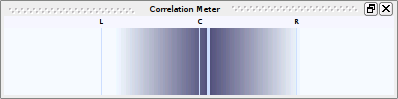
\includegraphics[width=0.7\textwidth]{images/cmeter1}}
	\subfigure[Mono, $r = 1.0$]{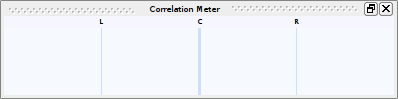
\includegraphics[width=0.7\textwidth]{images/cmeter2}}
	\subfigure[Phasenauslöschung, $r = -1.0$]{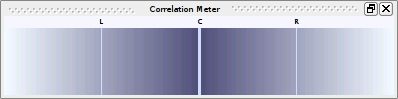
\includegraphics[width=0.7\textwidth]{images/cmeter4}}
	\caption{Die Korrelationsgradanzeige in Traverso zeigt den Korrelationskoeffizienten des Masterausgangs als Gradient zwischen zwei vertikalen Linien, die jeweils den linken und rechten Kanal darstellen. Verläuft der Gradient genau von L bis R, ist das Signal völlig unkorreliert ($r = 0.0$), und es besitzt ein sehr breites Stereobild (oben). Reduziert sich der Gradient auf eine Linie, sind die Daten perfekt korreliert ($r = 1.0$), was bedeutet, dass das Ausgangssignal mono erscheint (mitte). Erstreckt sich der Gradient über die L und R Linien hinaus, wird die Korrelation negativ und das Risiko von Phasenauslöschungen im Monosignal steigt an (unten).}
	\label{fig_cmeter01}
\end{figure}

Die Korrelationsgradanzeige kann auch dazu verwendet werden, die Balance des Signals zu justieren. Für ein zentriertes Signal, das auf beiden Kanälen etwa gleich laut klingt, sollte die Zenterlinie des Gradientes um die Mittenlinie herumtanzen.

Da sich der Gradient normalerweise zwischen den beiden Linien L und R befindet, kann man mittels \sact{M} den horizontalen Anzeigebereich verändern. Mehrmaliges drücken von \sact{M} setzt den Wert wieder auf den kompletten Bereich zurück.

\section{FFT-Spektrumsanzeige}
Eine auf der Fast Fourier Transformation (FFT) basierende Spektrumsanzeige gehört heutzutage zur Standardausrüstung einer digitalen Audioworkstation. Die FFT-Spektrumsanzeige in Traverso wird über das Menü ,,Ansicht $\rightarrow$ FFT-Frequenzspektrum'' aufgerufen. Sie wurde als Dock-Fenster realisiert, das man entweder in das Hauptfenster integrieren oder frei auf dem Bildschirm platzieren kann.

Die FFT-Spektrumsanzeige analysiert den Master-Ausgang und zerlegt das Audiosignal in Frequenzbänder. Jedes Band zeigt den höchsten Betrag $dB_{links} + dB_{rechts}$ innerhalb seines Bereichs (\FigB\ \ref{fig_fft1}). Ein Einstellungsdialog kann über den Befehl \sact{E} geöffnet werden, oder über das Kontextmenü \sact{Q}.

\begin{figure}
	\centering
	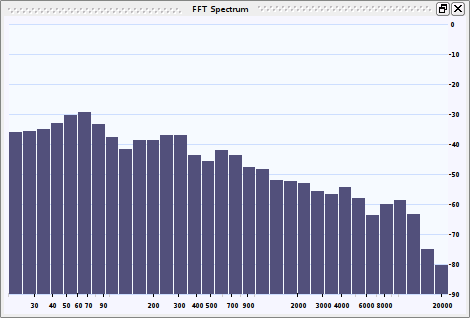
\includegraphics[width=0.6\textwidth]{images/fft1}
	\caption{Die FFT-Spektrumsanzeige zerlegt das Mastersignal in seine Frequenzen.}
	\label{fig_fft1}
\end{figure}

Der Konfigurationsdialog (\FigB\ \ref{fig_fft3}) ermöglicht es, den angezeigten Wertebereich in dB und Frequenzen zu definieren. Das für Menschen hörbare Spektrum reicht ungefähr von 20 bis 18000~Hz. CDs speichern einen Bereich von 20 bis 22050~Hz. Der angezeigte Frequensbereich sollte also in den meisten Fällen etwa diese Frequenzen abdecken. Für die Lautstärke gelten in der Regel eine Obergrenze von $-6$ bis $+6$~dB und eine Untergrenze im Bereich von $-60$ bis $-120$~dB. Die Anzahl Frequenzbänder kann frei gewählt werden, man sollte jedoch beachten, dass die Prozessorauslastung mit der Anzahl Bänder zunimmt, und ab $\geq 128$ erheblich werden kann.

Die Funktion ,,Durchschnittskurve anzeigen'' oder \sact{M} aktiviert eine Kurve, die während des Abspielens die gemessenen Frequenzen summiert und den Durchschnitt berechnet. Wird der Transport gestoppt und wieder gestartet, beginnt die Berechnung von neuem. Die Kurve kann auch durch drücken von \sact{L} zurückgesetzt werden. Sobald Durschnittswerte vorhanden sind, können diese auch exportiert werden. Als Exportformate stehen eine ASCII-Tabelle oder \texttt{grace} zur Verfügung. Letzteres kann mit dem Programm XmGrace geöffnet werden.

FFT-relevante Parameter können im Abschnitt ,,Erweitert'' im Einstellungsdialog geändert werden. Die Grö"se der FFT bestimmt die tiefste Frequenz, die von der Analyse noch erfasst wird. Je grö"ser die FFT, desto tiefer die Frequenz, aber desto höher wird die Speicher- und Prozessorbelastung. Die tiefste Frequenz wird wie folgt berechnet:
\[
f_{min} = \frac{\textrm{Samplerate}}{\textrm{FFT size}}
\]
Die \emph{tiefste} Frequenz bei einer FFT-Grö"se von 1024 Samples beträgt demnach bei einer Samplerate von 44100~Hz genau 43.1~Hz. Vergrö"sert man die FFT auf 2048 Samples, liegt die tiefste Frequenz bei 21.5~Hz. Die \emph{höchste} gemessene Frequenz berechnet man durch
\[
f_{max} = 0.5 \cdot \textrm{Samplerate}
\]
Für Audiodaten mit einer Samplerate von 44100~Hz liegt sie daher fest bei 22050~Hz.

Die Fensterungsfunktion kann in diesem Dokument nicht mit einfachen Worten erklärt werden, und es empfiehlt sich in den meisten Fällen, die ,,Hanning''-Funktion zu verwenden.

\begin{figure}
	\centering
	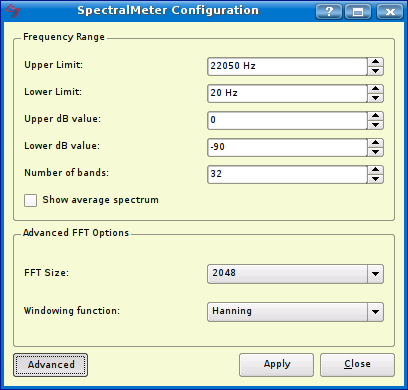
\includegraphics[width=0.7\textwidth]{images/fft3}
	\caption{Über einen Konfigurationsdialog (\sact{E}) kann man diverse Parameter einstellen.}
	\label{fig_fft3}
\end{figure}

\emph{Wichtig:} Für sehr grosse FFTs wird die Darstellung des Frequenzspektrums sehr ruckelig. Dies ist nicht unbedingt durch die erhöhte Prozessorbelastung bedingt, sondern durch die Tatsache, dass die FFT-Puffer einige Zeit brauchen, bis sie mit neuen Audiodaten gefüllt sind. In dieser Zeit wird das Spektrum nicht neu gezeichnet.

\section{Externe Bearbeitung}
Traverso bietet die Möglichkeit, Audioclips extern durch Zusatzprogramme wie ,,sox'' \cite{sox} zu bearbeiten. Dies ermöglicht die Verwendung von zusätzlichen Effekten, was besonders für Samplerate-Konversionen, Entfernung von Gleichspannung, Phaseninvertierung etc. geeignet ist. Auf Linux-Plattformen muss das Programm ,,sox'' installiert werden, das jedoch in allen gängigen Distributionen über das offizielle Repositorium verfügbar ist. Auf Windows und OS X wird das Programm mit Traverso automatisch installiert.

\begin{figure}
	\centering
	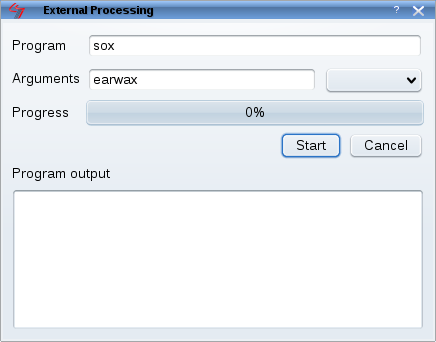
\includegraphics[width=\textwidth]{images/external00}
	\caption{Drückt man auf einem Audioclip \sact{E}, so öffnet sich ein Dialog (links). Drückt man darin den Knopf ,,Externe Bearbeitung'', öffnet sich ein weiterer Dialog (rechts), in dem man zahlreiche Effekte auf die Audiodatei anwenden kann.}
	\label{fig_external01}
\end{figure}

Ein Editor kann durch drücken von \sact{E} auf einem Audioclip geöffnet werden (\FigB~\ref{fig_external01}). Drückt man darin den Knopf ,,Externe Bearbeitung'', öffnet sich ein weiterer Dialog, in dem die Einstellungen dazu vorgenommen werden (\FigB~\ref{fig_external01} right). Lasst das ,,Programm'' jeweils auf ,,sox'' eingestellt, und wählt einen Effekt aus der ,,Argumente''-Box aus. Lasst den Namen des Argumentes in der Zeile stehen und hängt eure eigenen Argumente an. Verwirrt? Gut, dann betrachten wir ein Beispiel. Nehmen wir an wir wollen die Phase der Datei meinedatei.wav invertieren. Importiert sie dazu in Traverso und drückt \sact{E} auf dem Clip, danach den Knopf ,,Externe Bearbeitung'' im Bearbeitungsdialog. Lasst ,,sox'' als Programm eingestellt und wählt als Effekt ,,vol'' aus. Das erste Argument wird auf ,,vol'' gesetzt. Gemä"s der sox-Dokumentation invertiert man die Phase, indem man ,,vol'' auf $-1.0$ stellt. Schreibt also hinter das automatisch eingesetzte ,,vol'' noch ,,$-1.0$'' (ohne Anführungszeichen). Dann drückt ,,Start'' und wartet, bis der Prozess vorbei ist. Der Clip in Traverso wird automatisch durch die neue Wave-Datei ersetzt, die den Namen ,,meinedatei-vol -1.0.wav'' trägt. Die neue Datei wird im Verzeichnis ,,audiosources'' in eurem Projektverzeichnis gespeichert, unabhängig davon wo die ursprüngliche Datei lag. Durch die Umbenennung wird die Originaldatei nie überschrieben. Weitere Informationen zu sox-Effekten findet man in der man-page, die auf Linux durch Eingabe von ,,man:sox'' in Konqueror, oder ,,man sox'' in einem Terminal geöffnet wird.
\chapter{Getting Help\label{sect_help}}
There are several internet resources which can provide help if you struggle with Traverso. Before posting a question, however, it is recommended to carefully classify your problem. The source packages released by the Traverso team are usually well tested and compile without too much tinkering. If you still fail to compile it on your system, the Traverso team will most probably refer you to the user forum of your distribution. You can make life easier for all of us by posting your question there in the first place. Thus we ask you to consider the following points before asking for help.

\section{Compilation fails}
Please make sure that you have installed all required packages listed in chapter \ref{sect_installation} of this document. If you still get the error, search the archive of the Traverso developer mailing list \cite{ml-archive} for the same problem. If you don't find a solution, send an e-mail with a description  and the compiler output attached to the developer mailing list (traverso-devel@nongnu.org) or file a support request on the Savannah project page \cite{support}. Chances are high that the problem is distribution-specific and that you will be asked to refer to the user forum of your distribution.

If you can track down the error to missing dependencies, please consider to seek advice in the distribution forum in the first place.

\section{Binary package fails to install}
Search the archive of the Traverso developer mailing list \cite{ml-archive} for the solution. If you don't find the answer, send an e-mail with an accurate description of the problem to the Traverso developer mailing list (traverso-devel@nongnu.org).

\section{Bugs}
Search the archive of the Traverso developer mailing list \cite{ml-archive} and the bug tracker on Savannah \cite{bugtracker} for discussions of the problem. If you don't find any references, report the bug with instructions for reproduction, relevant information on your hardware, and the version of the Qt library used, on the bug tracker \cite{bugtracker}.

%\section{Feature request}
%Please (!) ask yourself if it is realistic to implement the requested feature at the current stage of development. If yes, send an e-mail with a detailed description to the developer mailing list \cite{ml-archive}.

\section{Getting involved}
The Traverso team highly appreciates any kind of contribution. If you are C++ coder, artist, musician, translator, or bug hunter who wants to help making Traverso the best multitrack application ever, please offer your help on the developer mailing list (traverso-devel@nongnu.org).


\chapter{Troubleshooting}
\begin{itemize}
 \item \textit{La reproducción es discontinua y obtengo muchos xruns}\\
  Si se usa un chip de sonido integrado de Intel, puede convenir ajustar el Número de Periodos a 3 en lugar de 2. Esto se hace en la página ``Driver'' de la ventana de Preferencias, o en la configuración de Jack (usualmente qjackctl).  

 \item \textit{No puedo escuchar el sonido}\\
  Si la reproducción parece funcionar (los VUmetros muestran señal) pero no puede escuchar sonido, compruebe si el driver activo es el ``Null''. Si es así cargue otro driver, por ej. ALSA en Linux o PortAudio en OS X o Windows, e intente de nuevo. Si está usando el driver Jack, asegúrese de que la salida de Traverso está conectada a una salida de hardware, como se describe en el capítulo \ref{sect_setup}.

 \item \textit{No puedo cargar el driver}\\
  Puede ser que el tamaño de buffer especificado en los ajustes del driver, sea muy grande para su tarjeta de sonido. Pruebe reduciendo un poco la latencia. También puede ser que el sistema de sonido esté bloqueado por otra aplicación o ``demonio''. Si usa KDE, asegúrese de que aRTs se apague automáticamente tras unos segundos, e intente terminar cualquier otra aplicación que bloquee la tarjeta de sonido.

 \item \textit{El ratón deja de moverse cuando pulso una tecla}\\
  Para evitar acciones indeseadas, algunos portátiles deshabilitan el touchpad mientras se pulsan teclas. Por supuesto, esto estropea completamente el concepto de selección blanda, pero afortunadamente puede deshabilitarse en la mayoría de los casos. Si está usando Linux, el demonio \texttt{mouseemu} controla esta función. Puede deshabilitar \texttt{mouseemu} ejecutando el comando 
  \begin{verbatim}
  sudo /etc/init.d/mouseemu stop
  \end{verbatim}
  y comprobar si el problema se resuelve, o bien puede editar el archivo de configuración \texttt{/etc/defaults/mouseemu} y cambiar el valor 300 de la línea \texttt{TYPING\_BLOCK="-typing-block 300"} a 0. Si hay un signo de comentario ``\#'' al principio de la línea, quítelo. Después reinicie \texttt{mouseemu} tecleando
  \begin{verbatim}
  sudo /etc/init.d/mouseemu restart
  \end{verbatim}

 Si está usando OS X, deshabilite la función ``ignorar acciones de touchpad accidentales'' en los ajustes del sistema.

 \item \textit{Traverso no puede poner la tarea de audio en prioridad de tiempo real}\\
 Algunas distribuciones Linux no permiten ajustar a prioridad de tiempo real las tareas de audio. Pero una prioridad demasiado baja puede producir xruns  e interrupciones durante la reproducción y la grabación. Para evitarlo, añada estas líneas al archivo \texttt{/etc/security/limits.conf}, o si las líneas ya existen, simplemente cambie los números:

\begin{tabular}{llll}
\texttt{@audio} & \texttt{-} & \texttt{rtprio} & \texttt{90}\\
\texttt{@audio} & \texttt{-} & \texttt{nice} & \texttt{-10}\\
\texttt{@audio} & \texttt{-} & \texttt{memlock} & \texttt{3000000}\\
\end{tabular}

Guarde el fichero y reinicie el ordenador.

\end{itemize}



%\appendix
%---------------- End of the document ---------------

\begin{thebibliography}{xx}
   \bibitem{trav-hp}http://www.traverso-daw.org
   \bibitem{trav-repo}deb http://www.traverso-daw.org binary-i386/
   \bibitem{pro-audio-wiki}http://proaudio.tuxfamily.org/wiki/
   \bibitem{suse-ref}http://packman.links2linux.org/package/traverso
   \bibitem{macports}http://www.apple.com/downloads/macosx/unix\_open\_source/macports.html
%   \bibitem{savannah-ref}http://savannah.nongnu.org/projects/traverso/
   \bibitem{ml-archive}http://lists.gnu.org/archive/html/traverso-devel/
   \bibitem{support}http://savannah.nongnu.org/support/?group=traverso
   \bibitem{bugtracker}http://savannah.nongnu.org/bugs/?group=traverso
   \bibitem{sox}http://sox.sourceforge.net
   \bibitem{forum}http://www.traverso-daw.org/forum/index.php
\end{thebibliography}

\end{document}
